\documentclass[../TST.tex]{subfiles}
\begin{document}
\begin{pproblem}
A half-cylinder of radius $r$ lies on the ground with its flat surface down. A uniform rod of rectangular cross section is placed symmetrically on top of the half-cylinder perpendicularly to its axis. The rod has mass $m$, length $l$, and height $h$. The acceleration due to gravity is $g$.
\begin{subpart}
	\item How should the parameters be related if the rod's equilibrium is stable?
	\item If the equilibrium is stable, find a formula for the oscillation period of the rod $T$ when it is displaced from its equilibrium position.The rod does not slip on the half-cylinder's surface.
\end{subpart}
\end{pproblem}
\ifprob \else
\begin{solution} (a) This is Problem 8.4 (`Leaning rectangle') from Morin's textbook. I will provide a solution of my own here. Let's place the coordinate origin $(x,y)=(0,0)$ at the centre of the half-cylinder. When the rod is in equilibrium, the centre of mass (CM) of the rod is at $(0,r+\frac{h}{2})$. Now let's rotate the rod along the cylinder so that it ends up at a small angle $\theta$ to the horizon. As this happens, the contact point between the two objects sweeps an arc $r\theta$ on the surface of the cylinder. Since there is no slipping, the objects' surfaces are essentially interlocked, so the total shift in the contact point's position is equal on both surfaces.  Thus, on the rod, the new contact point is shifted by exactly $r\theta$ with respect to the middle:
\begin{center}
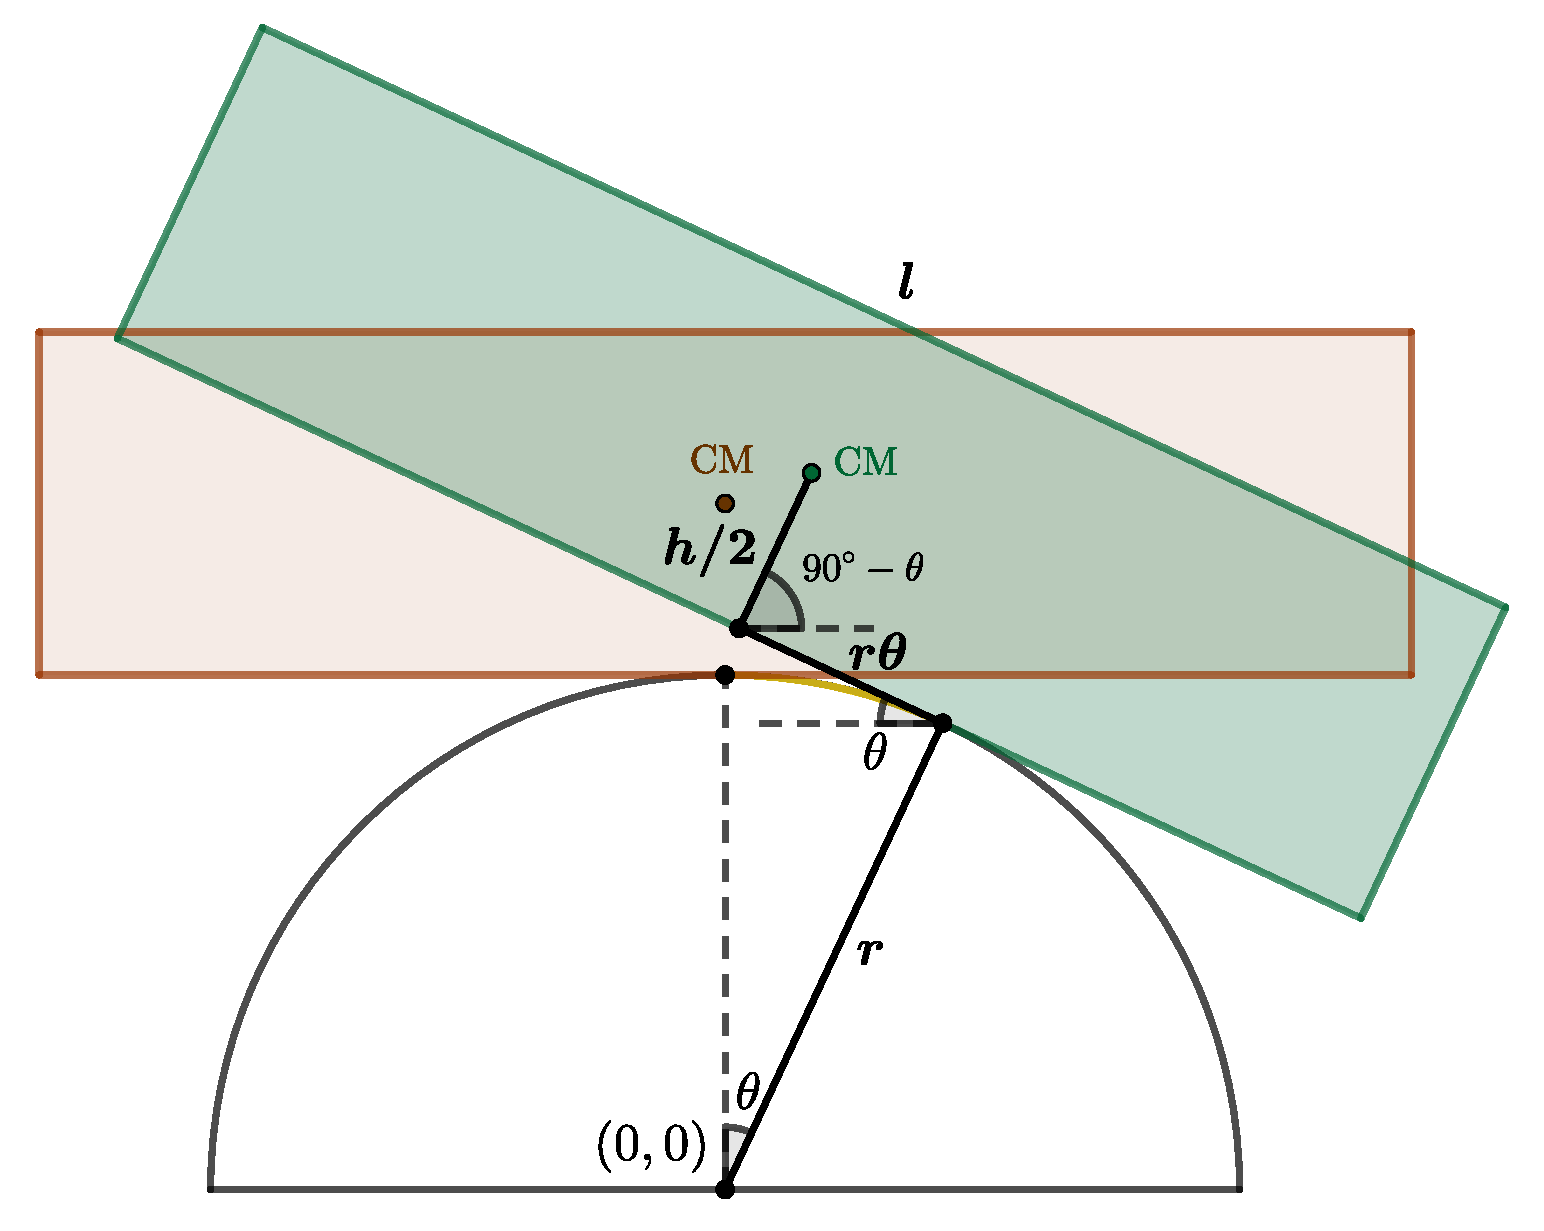
\includegraphics[width=0.7\textwidth]{fig/a2016_s1.pdf}
\end{center}
The position of the CM can then be described with
\begin{align*}
	x&=\left(r+\frac{h}{2}\right) \sin{\theta}-(r\theta)\cos{\theta},\\
	y&=\left(r+\frac{h}{2}\right) \cos{\theta}+(r\theta)\sin{\theta}.
\end{align*}
The shift of the CM's height, accurate to second order in $\theta$, is
\begin{equation*}
\Delta y = y-\left(r+\frac{h}{2}\right) \approx \left(r+\frac{h}{2}\right)\left(1-\frac{\theta^2}{2}\right) +r\theta^2-\left(r+\frac{h}{2}\right) = \frac{1}{2}\left(r-\frac{h}{2}\right) \theta^2,
\end{equation*}
and hence the potential energy, taking it as zero in equilibrium, is $E_p=mg\Delta y=\frac{1}{2}mg \left(r-\frac{h}{2}\right) \theta^2$. For the equilibrium of the rod to be stable, neighbouring configurations should have a higher potential energy, meaning that the term in front of the $\theta^2$ has to be positive. The condition for stable equilibrium is then \fbox{$r>h/2$}.\\

(b) The velocity of the centre of mass can be found by differentiating the expressions for its position:
\begin{align*}
	v_x&=\left( \left(r+\frac{h}{2}\right) \cos{\theta}-r\cos{\theta}+r\theta\sin{\theta}\right)\dot{\theta},\\
	v_y&=\left( -\left(r+\frac{h}{2}\right) \sin{\theta}+r\sin{\theta}+r\theta\cos{\theta}\right)\dot{\theta}.
\end{align*}
After applying the small-angle approximations, the only remaining large term is $v_x=\frac{h}{2}\dot{\theta}$. The kinetic energy of the rod can be broken up into a translational term $\frac{mv_\mathrm{CM}^2}{2}$ and a rotational term $\frac{I\dot{\theta}^2}{2}$, where the moment of inertia of the rod about its centre of mass is $I=\frac{1}{12}m(l^2+h^2)$, as derived in TST Problem 2012-2. In total, kinetic energy is 
\begin{equation*}
	E_k=\frac{1}{2}m \left(\frac{h^2}{4}+\frac{l^2}{12}+\frac{h^2}{12}\right)\dot{\theta}^2=\frac{1}{2}m \left(\frac{h^2}{3}+\frac{l^2}{12}\right)\dot{\theta}^2
.
\end{equation*}
Next, given that total energy (which has the form $A\dot{\theta}^2+B\theta^2$) is a conserved quantity, we can differentiate it to find the equation of motion of the rod:
\begin{equation*}
	\frac{\mathrm{d}}{\mathrm{d}t}\left(E_k+E_p\right)= \frac{\mathrm{d}}{\mathrm{d}t}\left(A\dot{\theta}^2+B\theta^2\right) = 2\dot{\theta}\left(A\ddot{\theta}+B\theta\right)=0
.
\end{equation*}
Setting the stuff in the parentheses to zero, we get simple harmonic oscillations with an angular frequency $\omega =\sqrt{\frac{B}{A}}$. In this problem we have $A=\frac{1}{2}m \left(\frac{h^2}{3}+\frac{l^2}{12}\right) $ and $B=\frac{1}{2}mg \left(r-\frac{h}{2}\right) $, so the period is
\begin{equation*}
	T=\frac{2\pi}{\omega}=\boxed{2\pi\sqrt{\frac{4h^2+l^2}{6g(2r-h)}}.}
\end{equation*}

\end{solution}
\fi
\end{document}
